

\subsection{Transcript Generation and Computing Verifier Challenges}\label{sec:transcript-gen}

We will describe our protocol version as a non-interactive protocol using the Fiat-Shamir heuristic \cite{C:FiaSha86}. Therefore, we need to specify how we are generating the random challenges from $\KK$ (or equivalently, $3$ elements of $\FF$). Throughout this section, we will use an instance of a Poseidon hash function having a state size of $12$ field elements ($8$ for inputs and $4$ for capacity) and an output size of $12$ field elements. 

The strategy for generating the transcript is similar to the linear hash strategy described before. Suppose we want to add $c_1, \dots, c_r$ elements to the transcript. We proceed as follows:

\begin{enumerate}

\item The input is split in chunks of $8$ field elements, filling with repetitions of the $0$ element if $r$ is not a multiple of $8$. 

\item The first chunk is hashed using Poseidon with capacity $(0,0,0,0)$.

\item The following chunk is hashed using Poseidon with the capacity being the $4$ last elements of the output of the previous hash. 

\item Go to Step $3$ until there are no more chunks. 

\end{enumerate}

Observe that the $8$ remaining elements of each hash output are not being used until we stop the loop between the steps $3$ and $4$. We depict the previous strategy in Figure \ref{fig:transcript-gen}.  

\begin{figure}[h!]
\centering
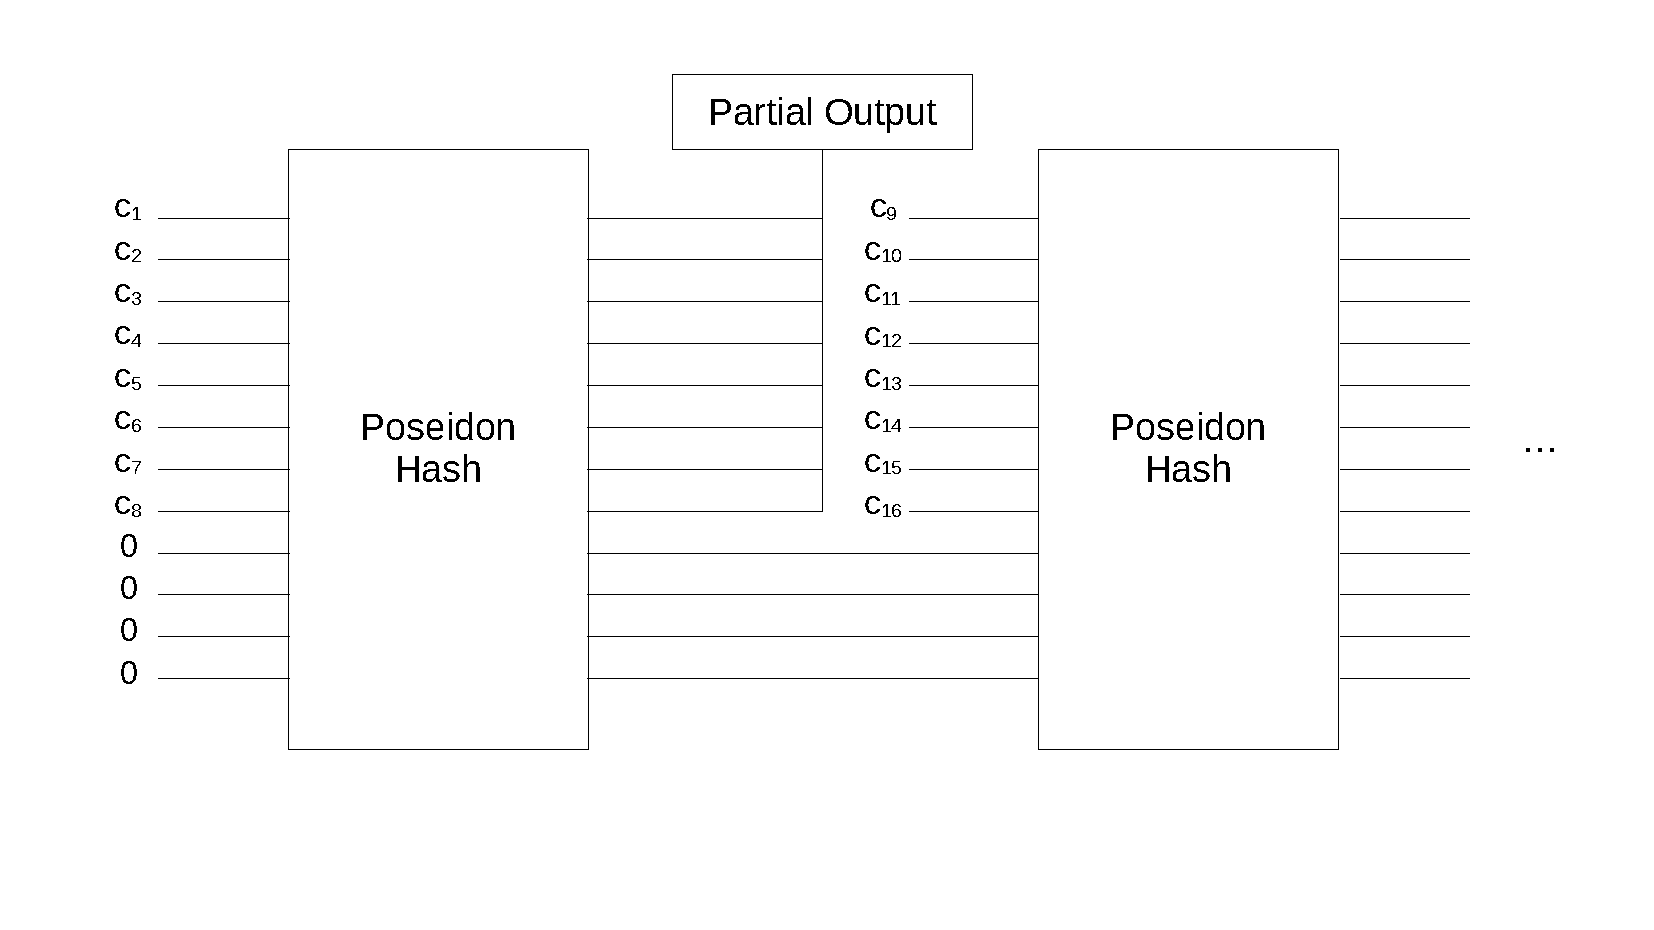
\includegraphics[width=.8\textwidth]{../figures/transcript}
\caption{First two steps of the transcript generation.}
\label{fig:transcript-gen}
\end{figure}

%TODO: Discuss it with Marc
%TODO: I think we should hash the entire previous output instead of zeros to obtain as many values as we need
When we stop adding elements to the transcript, we end up with an output consisting of $8$ field elements, say $(t_1, \dots, t_8)$. For a given transcript state we can extract as many challenges from $\KK$ as we need. The first two elements are trivially obtained
\[
t_1 + t_2 \varphi + t_3 \varphi^2, \quad t_4 + t_5 \varphi + t_6 \varphi^2
\]
for $\varphi$ being a root of the irreducible polynomial used to construct $\KK$ from $\FF$. Since we do not have enough elements to construct a third extension field element, we proceed as follows. We construct a field element $t_9$ hashing $8$ zeros with the capacity being the last $4$ output elements of the last hash performed at the time of generating the transcript (that is, the elements that will become the capacity of the next hash when adding a new element into the transcript). Hence, we get a third element in $\KK$
\[
t_7 + t_8 \varphi + t_9 \varphi^2.
\]
By 

We will denote by \transcript the transcript instance and we will define for it the following operations:

\begin{itemize}

\item \textbf{Add:} Having elements $c_1, \dots, c_r \in \FF$, we denote by 
\[
\transcriptAdd(c_1, \dots, c_r)
\]
the operation of adding $c_1, \dots, c_r$ to the transcript using the previous procedure. 

\item \textbf{Extract:} Having a transcript state \textsf{T}, we denote by
\[
\transcriptExtract{i}(\transcript) \in \KK \quad i \in \{1, 2, 3\}
\]
the result of extracting a single extension field $\KK$ element from it using the previously described procedure. Using the notation above:
\begin{align*}
&\transcriptExtract{1}(\transcript) = t_1 + t_2 \varphi + t_3 \varphi^2, \\
&\transcriptExtract{2}(\transcript) = t_4 + t_5 \varphi + t_6 \varphi^2, \\
&\transcriptExtract{3}(\transcript) = t_7 + t_8 \varphi + t_9 \varphi^2.
\end{align*}
\end{itemize}

A proof that the resulting non-interactive protocol is knowledge sound after applying the Fiat-Shamir using this strategy can be found, for example, in Theorem 4 of \cite{EPRINT:AttFehKlo21}.
